\documentclass[aspectratio=169,usenames,dvipsnames]{beamer}


\usetheme{default}  % You can choose any other theme you prefer

\title{06 - Algoritmos}
\subtitle{Interseção de Segmentos}
\author{Mateus Oliveira de Figueiredo}
\date{10/10/2023}

\usepackage{tikz}
\usetikzlibrary{matrix}
\usepackage{multicol}
\usepackage{algorithm}
\usepackage{algpseudocode}
\usepackage{xcolor}
\usepackage[utf8]{inputenc}
\usepackage[portuguese]{babel}
\usepackage{amsmath} % for "pmatrix" environment  

\usepackage{pgfplots}
\DeclareUnicodeCharacter{2212}{−}
\usepgfplotslibrary{groupplots,dateplot}
\usetikzlibrary{patterns,shapes.arrows, positioning}
\pgfplotsset{compat=newest}

\begin{document}

\begin{frame}
\titlepage
\end{frame}

\begin{frame}
\frametitle{Algoritmos Implementados}
\vfill
\begin{itemize}
  \item Força Bruta ({\it{Naive}})
  \item Algoritmo de Bentley-Ottmann
\end{itemize}
\vfill
\end{frame}

\foreach \n in {0,...,14} {
\begin{frame}
\frametitle{Algoritmo de Bentley-Ottmann}
    \begin{figure}
      \includegraphics[width=0.6\textwidth]{figs/event_\n.pdf}
    \end{figure}
\end{frame}

}

\begin{frame}{Estruturas de Dados}
  
  \vfill
  Para guardar os segmentos que estão ativos:
  \begin{itemize}
    \item Lista Ordenada
    \item Lista Não Ordenada
    \item Árvore Binária
  \end{itemize}

  \vfill
  Lista de eventos no caso de detecção de interseção foi usado uma lista.

  \vfill
\end{frame}

\begin{frame}{Exemplos Randomizados}
  \begin{columns}
    \begin{column}{0.5\textwidth}
      \begin{figure}
        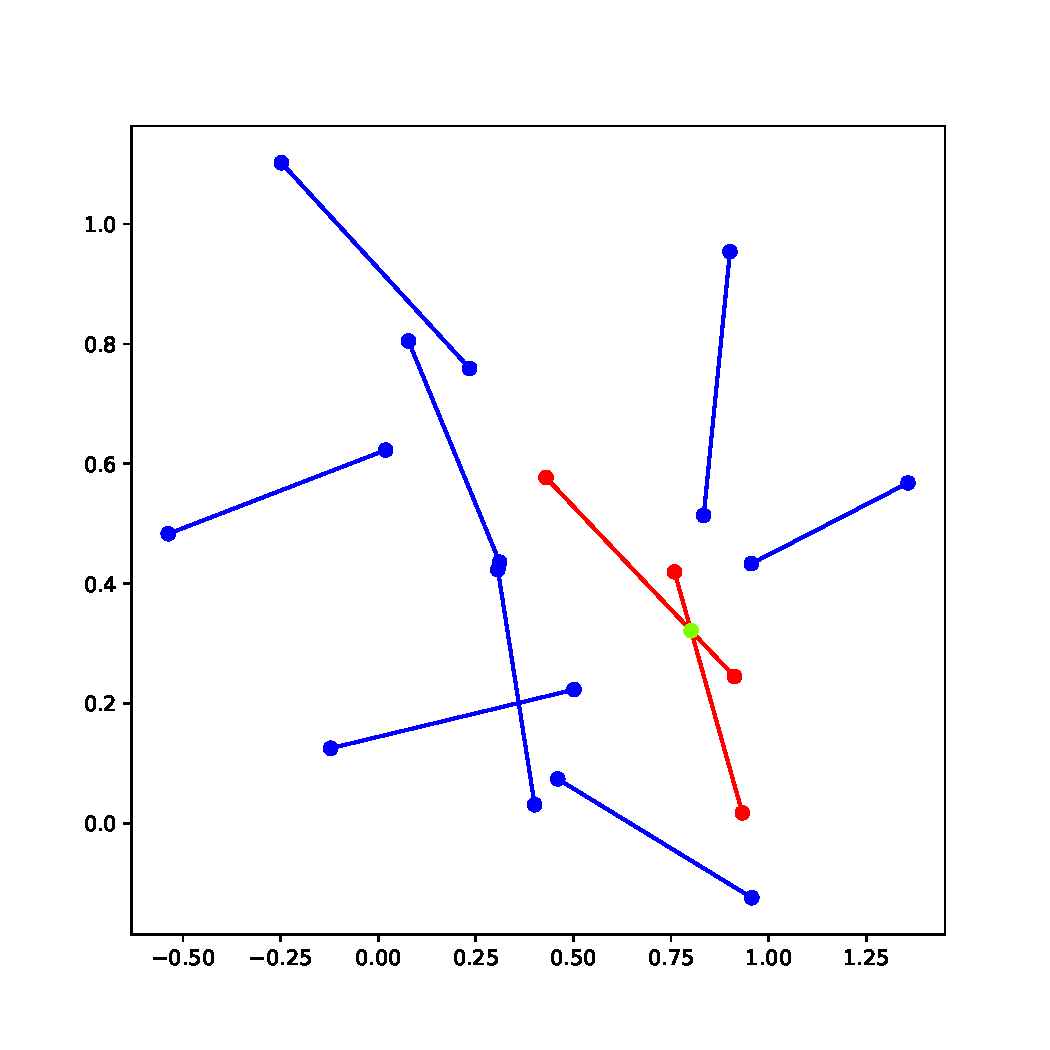
\includegraphics[width=0.9\textwidth]{figs/examples_0.pdf}
        \caption{10 Segmentos Sorteados}
      \end{figure}
    \end{column}
    \begin{column}{0.5\textwidth}
      \begin{figure}
        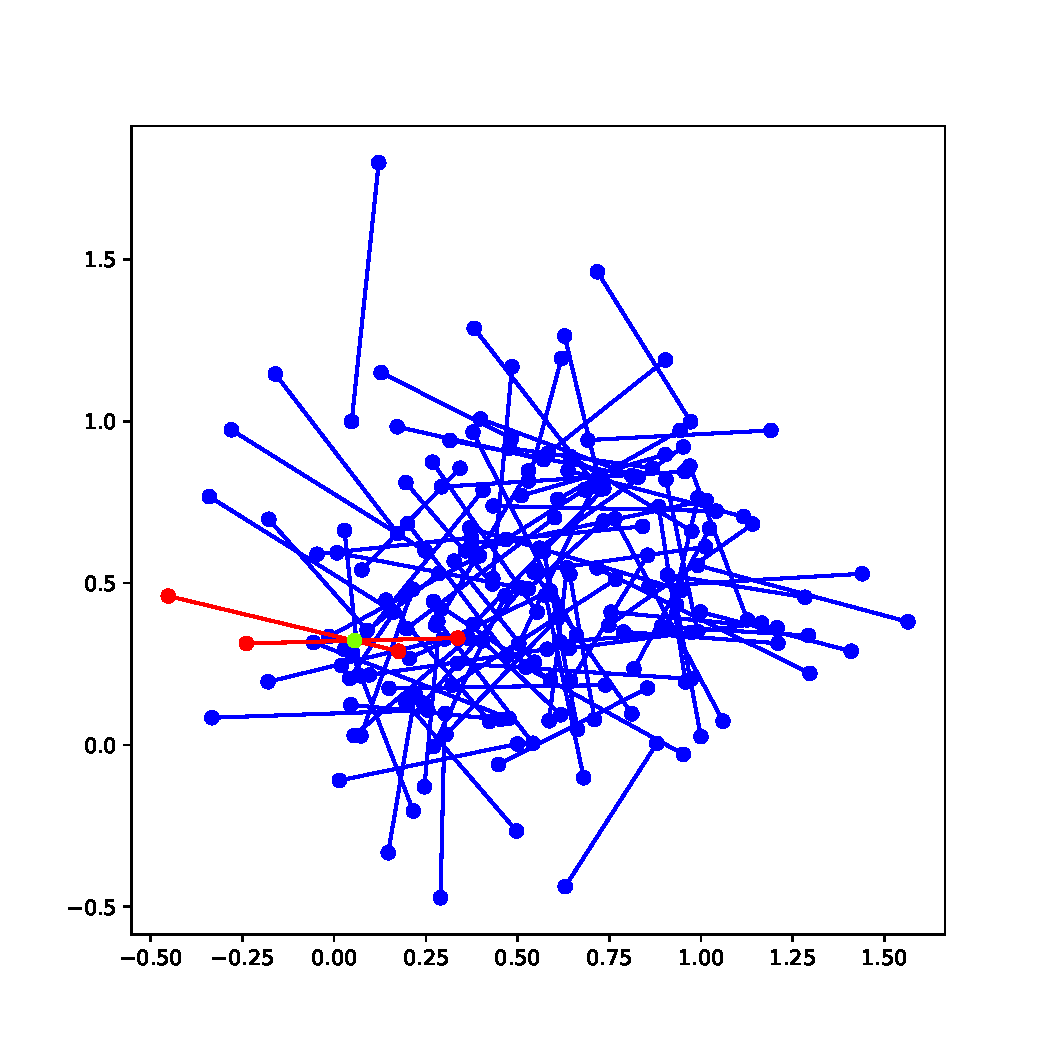
\includegraphics[width=0.9\textwidth]{figs/examples_1.pdf}
        \caption{100 Segmentos Sorteados}
      \end{figure}
    \end{column}
  \end{columns}
\end{frame}

\begin{frame}{Exemplos Sem Interseção - Segmentos Grandes}
  % Two columns
  \begin{columns}
    \begin{column}{0.35\textwidth}
      \begin{figure}
        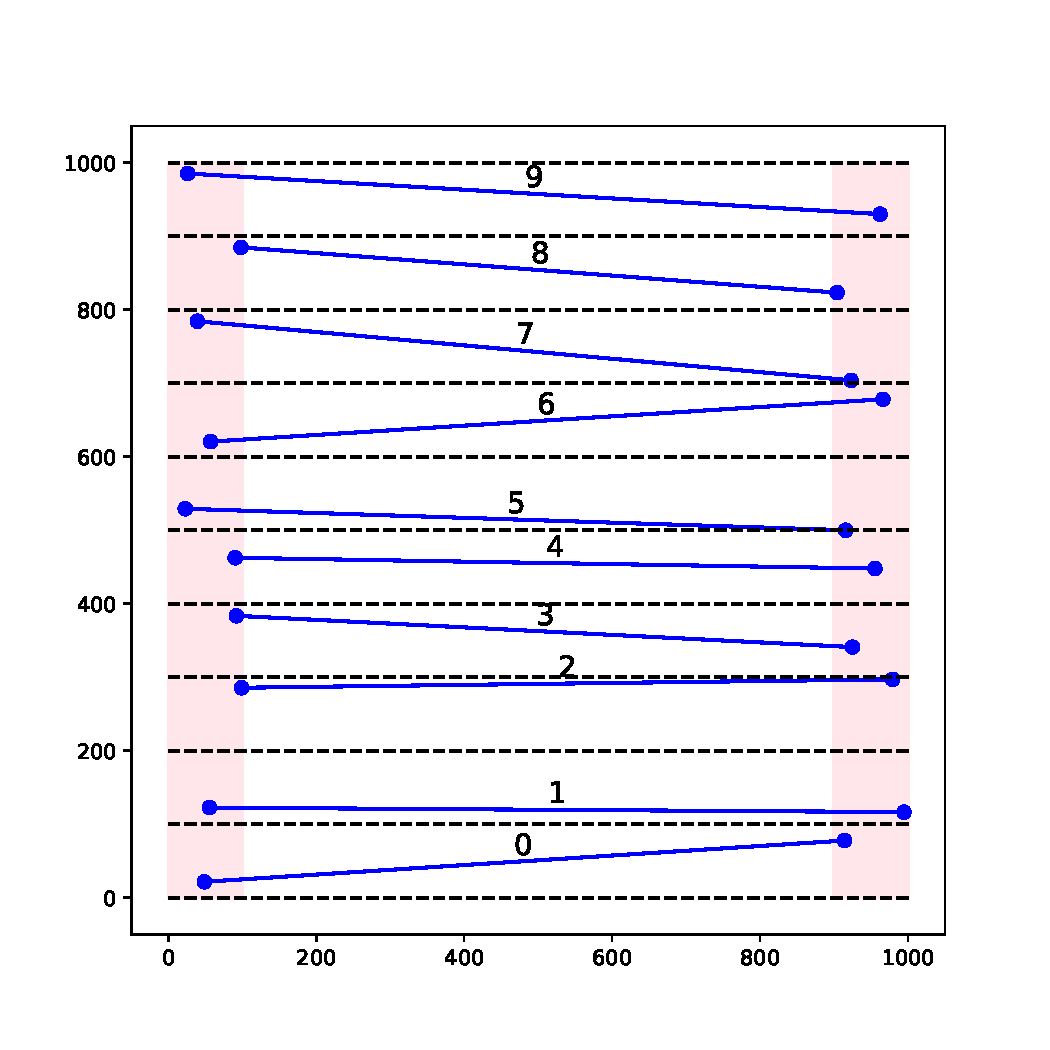
\includegraphics[width=\textwidth]{figs/big_example.pdf}
      \end{figure}
    \end{column}
    \begin{column}{0.65\textwidth}
      \begin{figure}
        \onslide<2>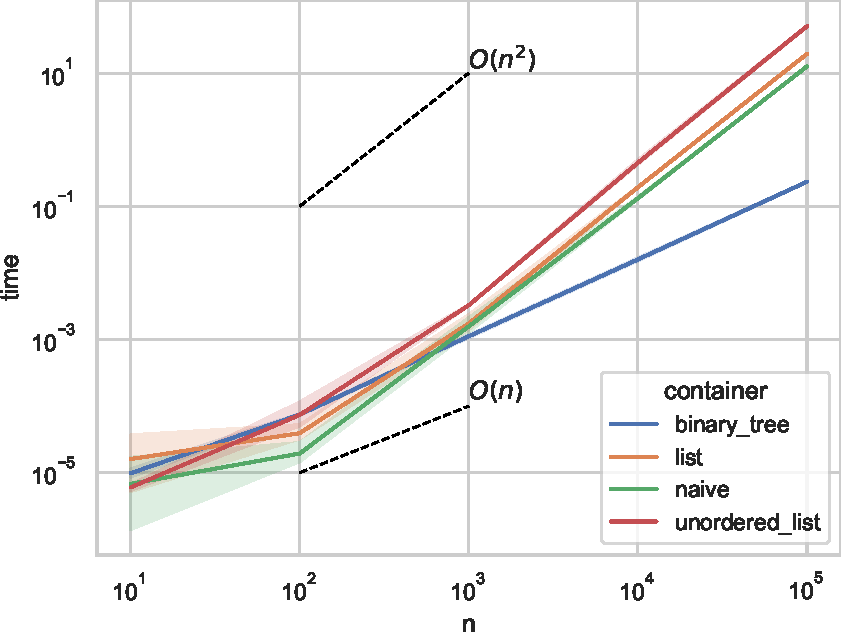
\includegraphics[width=0.9\textwidth]{figs/tests_big_segments.pdf}
      \end{figure}
    \end{column}
  \end{columns}
\end{frame}


\begin{frame}{Exemplos Sem Interseção - Segmentos Pequenos}
  % Two columns
  \begin{columns}
    \begin{column}{0.35\textwidth}
      \begin{figure}
        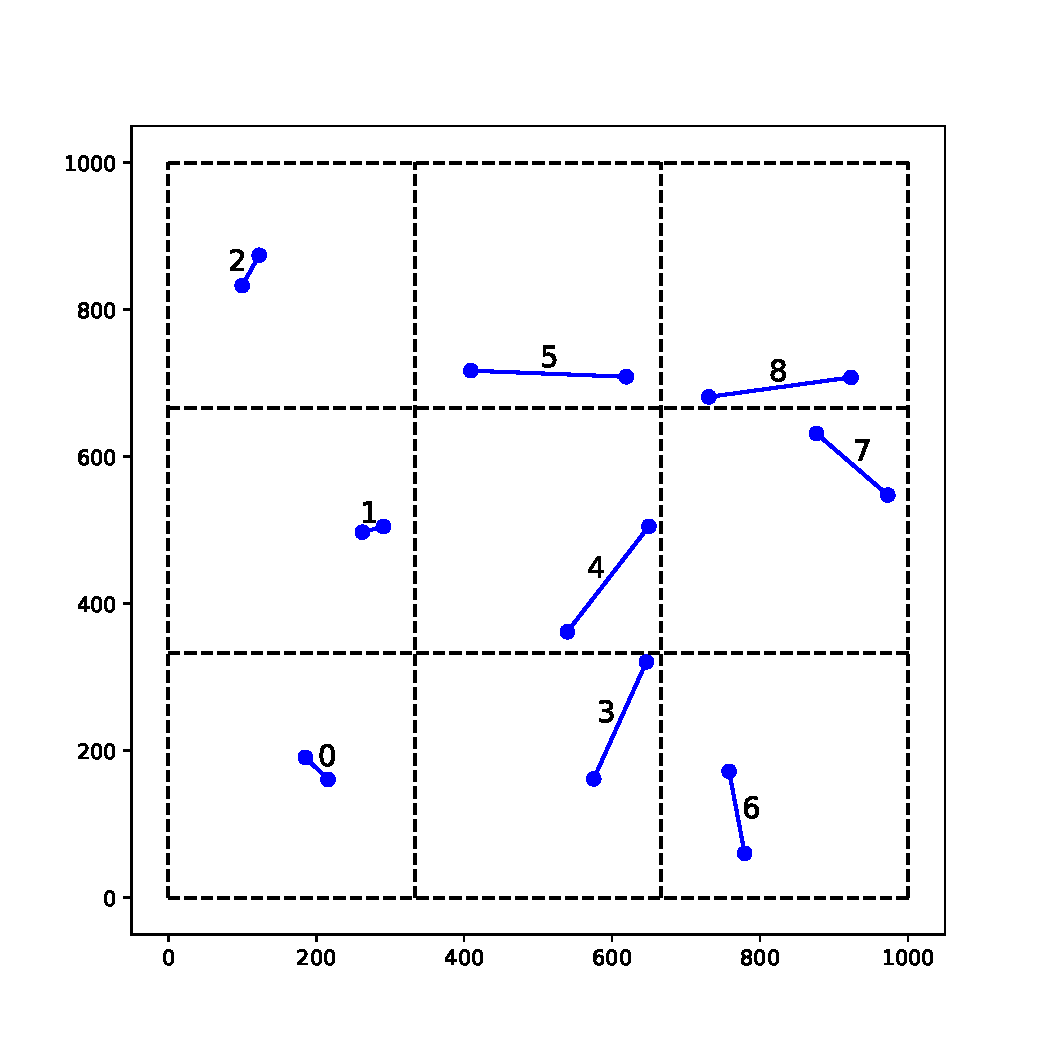
\includegraphics[width=\textwidth]{figs/box_example.pdf}
      \end{figure}
    \end{column}
    \begin{column}{0.65\textwidth}
      \begin{figure}
        \onslide<2>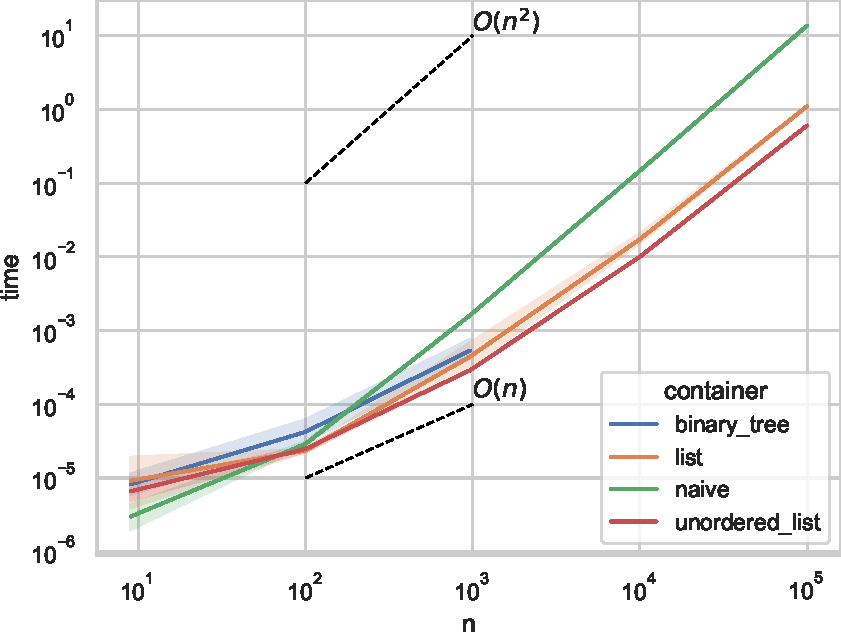
\includegraphics[width=0.9\textwidth]{figs/tests_box.pdf}
      \end{figure}
    \end{column}
  \end{columns}
\end{frame}

\begin{frame}{Comparação dos Pequenos x Grandes}
  % Two columns
  \begin{figure}
    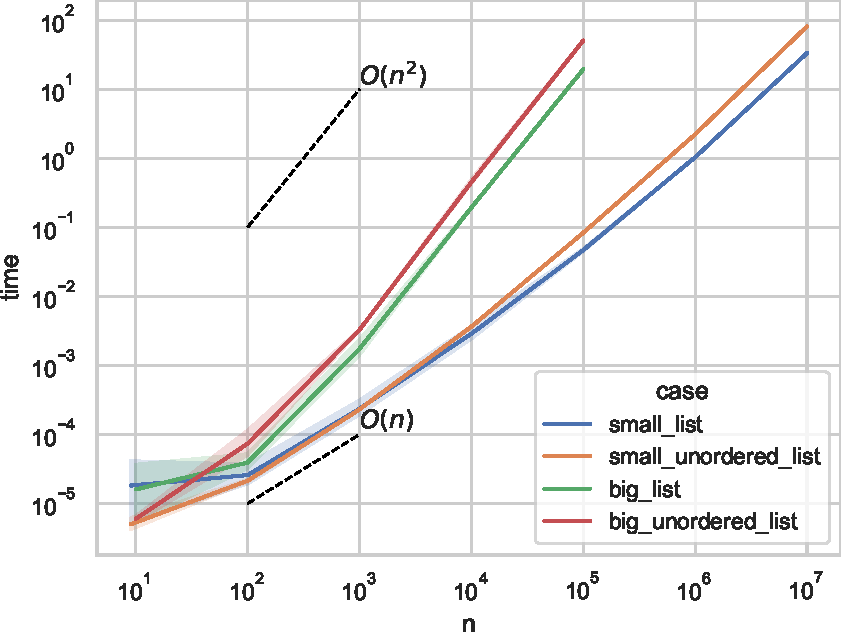
\includegraphics[width=0.7\textwidth]{figs/comp_cases.pdf}
  \end{figure}
\end{frame}


\end{document}